%%
%% Time-stamp: <2022-01-25 15:59:13 stefan>
%%
%% En CV i ett två-kolumn format
%%
%% Inspirerad av Kevin Fox (@fury.com) CV
%%

\documentclass[a4paper,swedish,10pt]{article}

\usepackage[utf8]{inputenc}

% fet för rubriker
\usepackage{tgadventor}

% brödtext
\usepackage[scaled=1.0]{gillius2}
\renewcommand*{\familydefault}{\sfdefault}

% specialfont för årtal
\usepackage{cinzel}
\usepackage[T1]{fontenc}    %% annars fungerar inte klipp-och-klistra från PDF självt

\usepackage{calc}
\usepackage{babel}
\usepackage[a4paper,top=2cm,bottom=2cm,left=1.5cm,right=1.5cm]{geometry}
\usepackage{fullminipage}
\usepackage{xcolor}
\usepackage{graphicx}
\usepackage[export]{adjustbox}
%% \usepackage{ragged2e}
\usepackage{enumitem}
\usepackage{blindtext}
\usepackage{adjustbox}
\usepackage[colorlinks=true, allcolors=blue]{hyperref}

\usepackage{fancyhdr}
\setlength{\headheight}{35pt}
%\addtolength{\topmargin}{-22pt}
\fancyhf[LH]{Stefan Skoglund\\Högalidsgatan 36\\521 61 Stenstorp}
\fancyhf[CH]{%
  stefan.skoglund@agj.net\\%
  \href{http://www.linkedin.com/in/stefan-niskanen-skoglund-902aa0a1}{Linkedin:Stefan Skoglund}\\
  \href{https://github.com/Skaraborgfakir}{github: Skaraborgfakir}}
\fancyhf[RH]{%
  0500--450 878\\0702--719 835
}
\fancyhf[CF]{\href{https://skaraborgfakir.github.io/cv_minipage_eng_2022.pdf}{URL for this CV version}}
\pagestyle{fancy}

\newenvironment*{descriptioncv}[1]%
{%
  \textbf{\large #1}%
  \begin{description}[nosep,font=\sffamily\bfseries, leftmargin=0.5cm, style=nextline]%
  }%
  {\end{description}\vspace{0.4cm}}
\newcommand*{\cvitem}[3]{\item[#1]{\cinzel#2}\\#3}

% DEBUG:utmatning av uppgifter om storlekar,kerning osv
\showoutput
\begin{document}

\begin{minipage}[t]{0.73\textwidth}
  \begin{descriptioncv}{Utbildningar och separata kurser}
    \cvitem{Lexicon, Göteborgs}{December 2021}{AZ900 certification}
    \cvitem{Lexicon, Göteborgs}{June 2021-December 2021}{Courses in programming in .Net. The curriculum included JavaScript,C\#, HTML, CSS, Azure and Entity Framework with Identity server}
    \cvitem{Lexicon, Göteborgs}{Mars 2021}{Qualified to Lexicon'ss Test\&Bedömning before enrolling in either of their user support or .Net course}
    \cvitem{History A, University of Gothenburg}{January-- Juni 2018}{Beginning courses in history}
    \cvitem{History B, University of Gothenburg}{August-- December 2018}{courses in historia, In my treatise, i used as a a source, a Umeå priest's own biography }
    \cvitem{Script programming in Linux, University of Gothenburg}{Våren 2019}{telemetry on Linux using \texttt{awk} and \texttt{bash} as programming languages, part of a telemetry program at Chalmers}
    \cvitem{Vocational trainiing as a railway signalling tech, Lärcenter Falköping}{August 2014--June 2015}{Focused on ERTMS. Including normal subjects in a railway tech area (points, track circuits, level crossing's control, relay based interlockings and IP based communication between interlockings and it's controlling centers (EBISAT) }
    \cvitem{Database technology A, University of Skövde}{2019}{Database design using UML, ER and MySQL}
    \cvitem{Computer networks A, Högskolan i Skövde}{2019}{CISCO ICND1}
    \cvitem{Linux administration A, Högskolan i Skövde}{2014}{UNIX admin: integrated email services with web front}
    \cvitem{UNIX B, Högskolan i Skövde}{2012}{UNIX admin: epost med web:gränssnitt}
    \cvitem{C:programming, Högskolan i Skövde}{1993}{The C computer language}
    \cvitem{Modellering, Högskolan i Skövde}{2018}{UML with group oriented business process modelling}
  \end{descriptioncv}
  \begin{descriptioncv}{Arbeten}
    \cvitem{Signalling tech, NVBS}{2017 Maj-- Augusti}{Contract work for renewal and new-build of relay based interlocking in Stockholm. Preparation work for the future
      bridge replacements between Centralstationen and Södra station.}
    \cvitem{Signalling tech, NVBS}{2016 Juli}{Contracted out as a signal maintaineer in Stockholm.}
    \cvitem{Signaltekniker, NVBS}{2015 Juli-- Augusti}{Contracted out as a maintaineer in Stockholm.}
  \end{descriptioncv}
\end{minipage}%
\begin{minipage}[t]{0.24\textwidth}%
  \raggedleft%
  \vspace{-\topskip+1cm}
  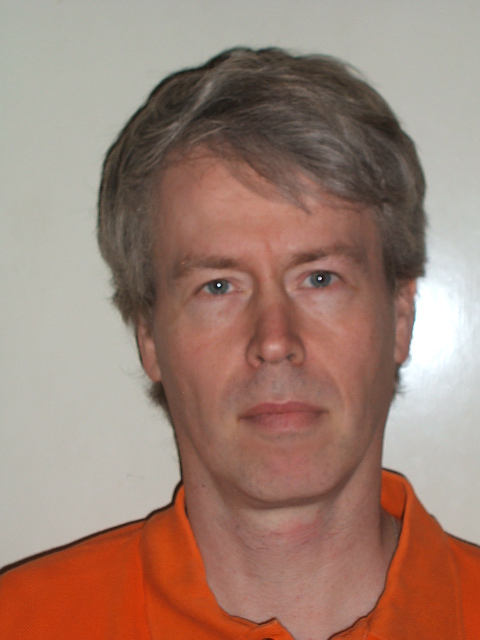
\includegraphics[height=3.5cm]{idbild.jpg}
  % 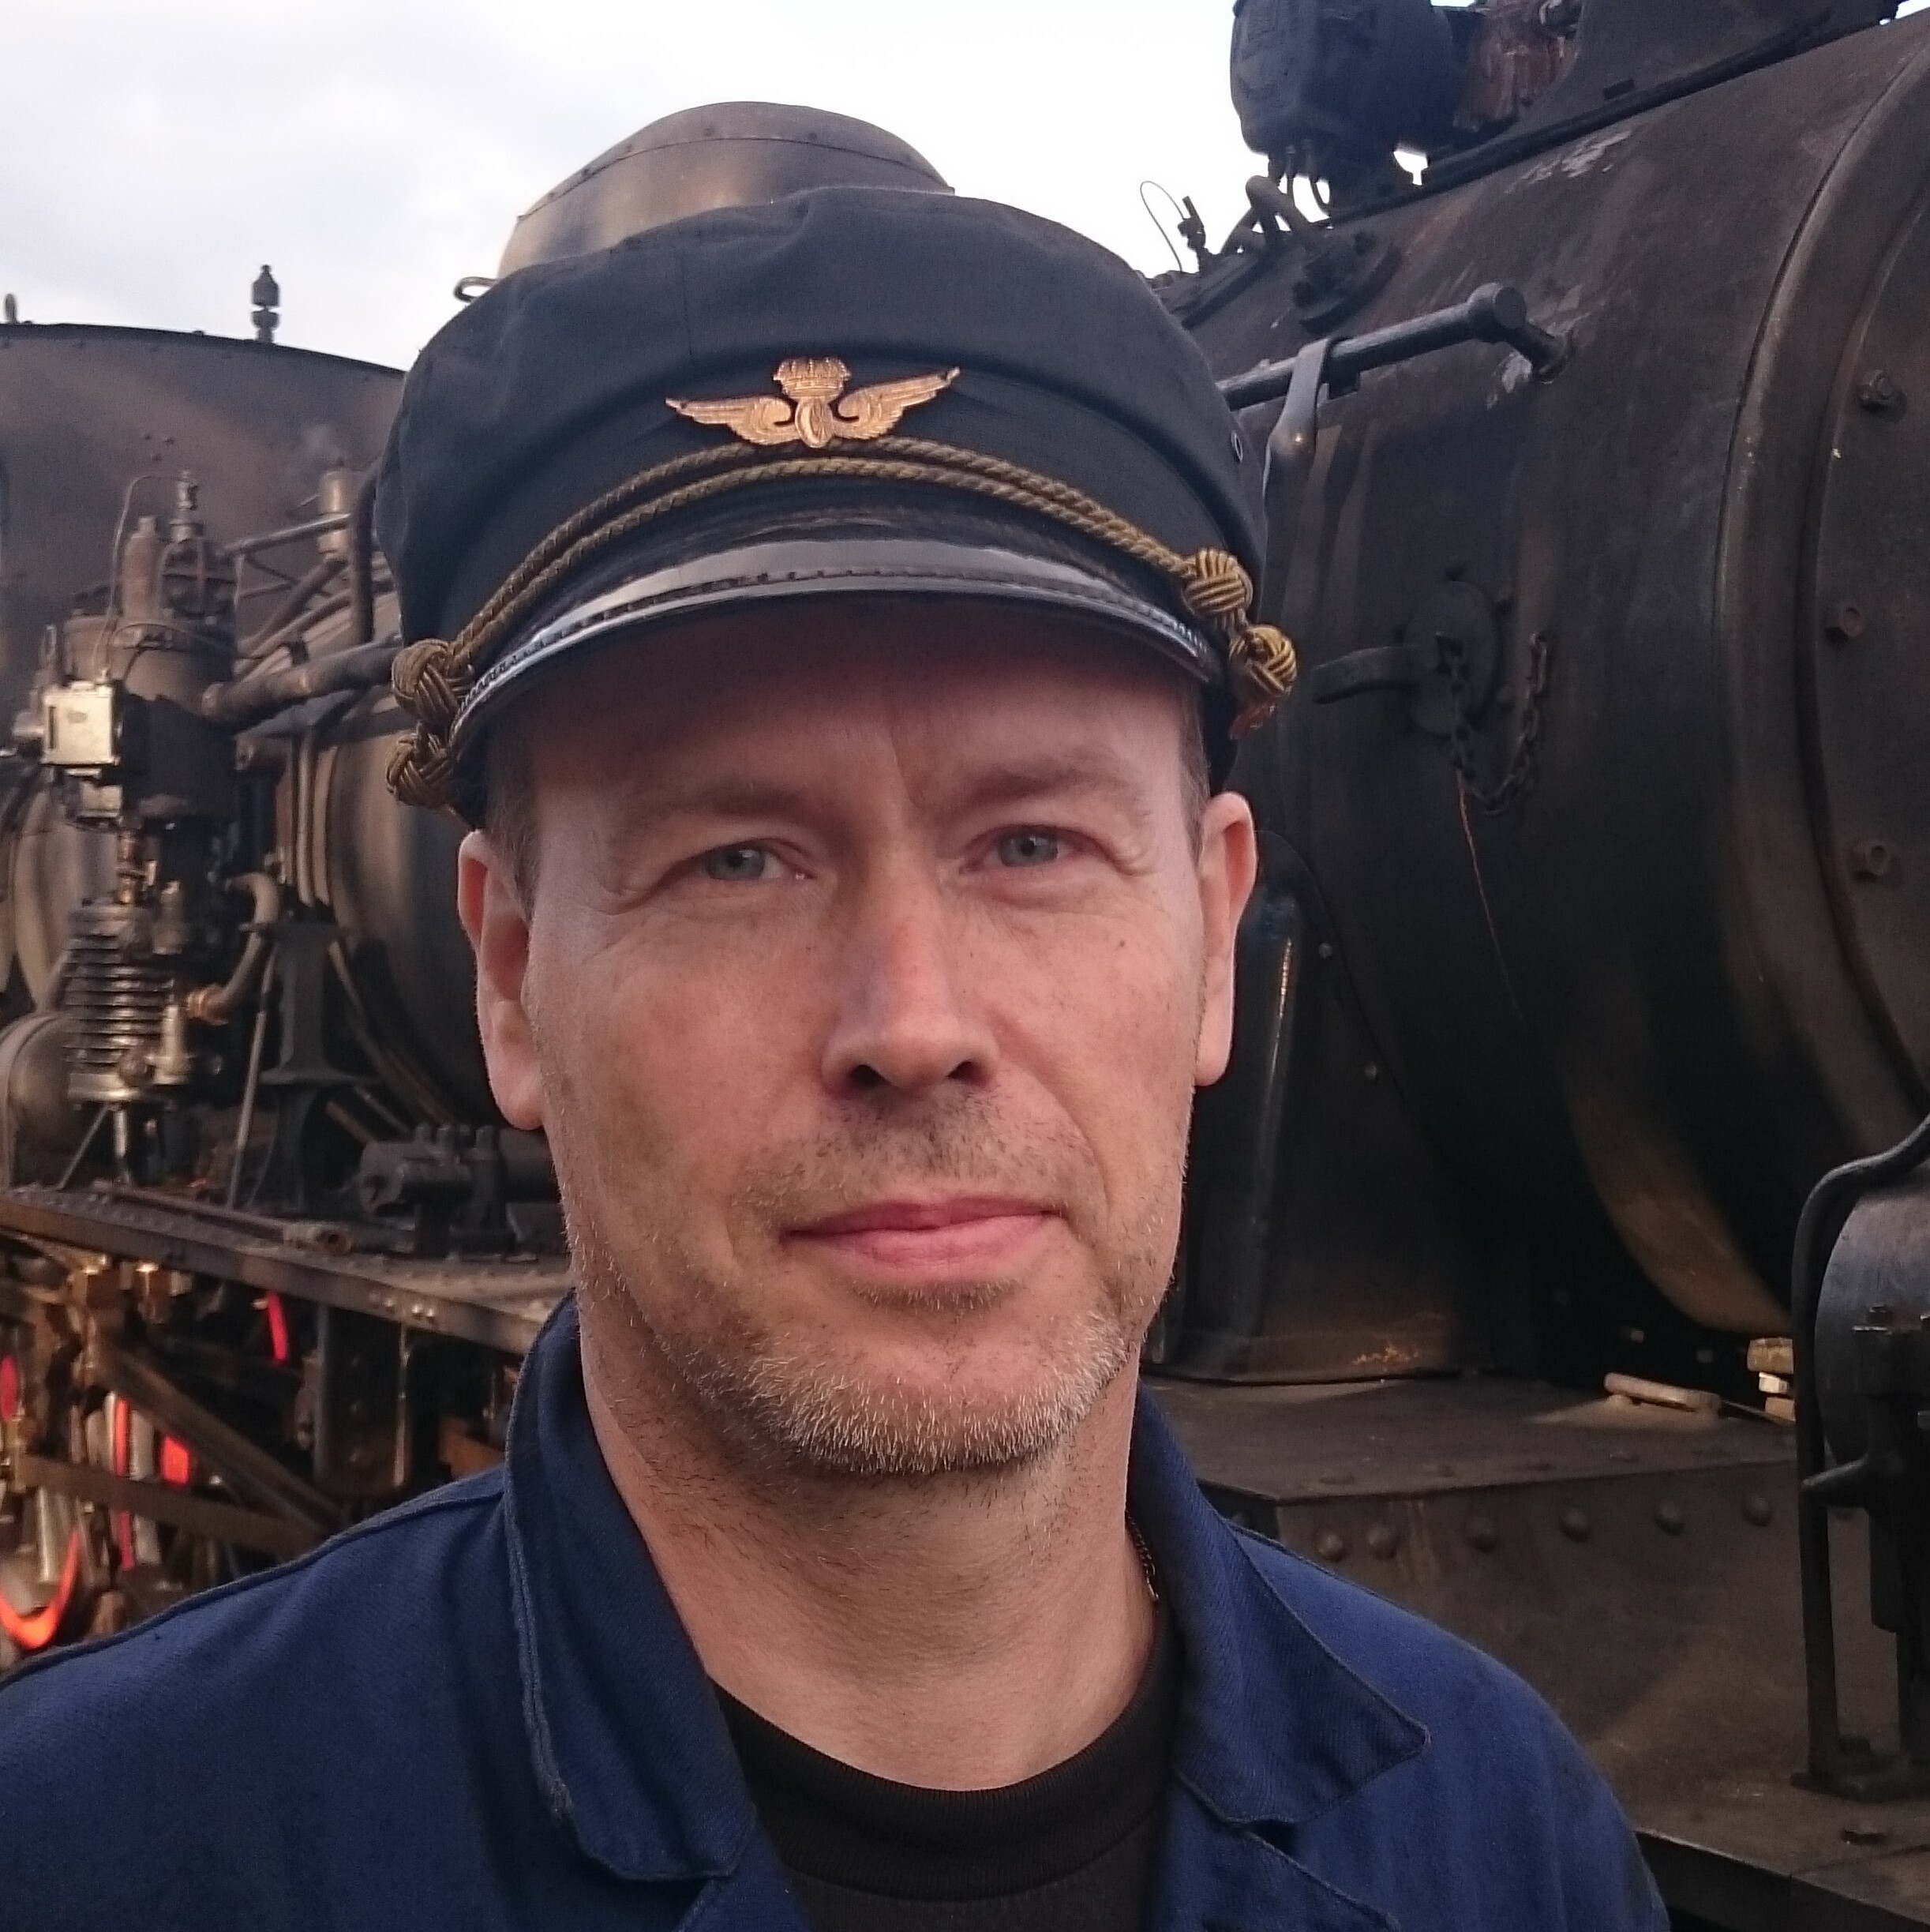
\includegraphics[height=3.5cm]{bild.jpg}
  \textbf{Development methods}
  \begin{description}[nosep]
    \raggedleft\setlength\itemsep{0.1ex}\small%
  \item Object-oriented programming
  \item Man-Machine interaction (MMI)
  \item UML
  \item C/C++
  \item Pascal
  \item Ada
  \item Python
  \end{description}
  \vspace{0.5cm}
  \textbf{Linux}
  \begin{description}[nosep,font=\sffamily\bfseries]
    \raggedleft\setlength\itemsep{0.1ex}\small%
  \item CFEngine (2012--)
  \item LINUX (RedHat 5 1997--)
  \item LINUX (Debian 2008--)
  \item Solaris (SunOS4/SunOS5)
  \item PostgreSQL
  \item Computer networks
  \item VMWare ESXi/vSphere (used in computer system courses)
  \item NexentaStor (deployed as a SAN/NAS to distribute, via iSCSI VMDK to a ESXi host. NFS for user folders)
  \end{description}
  \vspace{0.5cm}
  \textbf{Språk}
  \begin{description}[nosep,itemsep=0.1ex]
    \raggedleft\small%
  \item Swedish (mother tongue)
  \item Engelska (in speech and textual, excellent understanding)
  \end{description}
\end{minipage}

\begin{minipage}[t]{0.73\textwidth}
  \begin{descriptioncv}{Arbeten}
    \cvitem{Praktik, Infranord Herrljunga}{2015 Mars--Juni}{Internship as a signalling maintaineer, Herrljunga}
    \cvitem{Praktik, Infranord Stockholm}{2014 October}{Internship as a signalling maintaineer, Hagalund Stockholm}
    \cvitem{Servicetekniker, Kronbergs hushållsservice, Skövde}{Mars 1996--November 2006}{reparation av
      vitvaror (spisar,tvättmaskiner och småapparater) och frånluftsvärmepumpar.
      Kundkontakt med planering av arbeten. Försäljning av ersättningsmaskiner. Justering
      av ventilationssystem.}
    \cvitem{Telefonist, F6 Karlsborg}{1989-1990}{Miltex, försvarets fjärrskriftsystem. Flygvapnets system för kommunikation inom flygbaser}
  \end{descriptioncv}

  \begin{descriptioncv}{My own programming projects}
    \cvitem{PKI functionality}{2014--}{Automated deployment of certificates
      for a multi-tiered certification functionality.
      Consisting of a root certification issuer, one delegated intermediate issuer and multiple
      CAs whose own certificate is signed by the intermediate and which has a specific usage area, for example
      signing a individual person own certificate while another CA is limited to only signing
      certificates for a service, for example IMAP. }

    \cvitem{Automation of BIND}{2015--}{Automated configuration of ISC's BIND9 daemon.
      Uses descriptions formatted as JSON to generate zone descriptions.
      Including correctly updating a specific zones serial number when the zone's data is updated.}

    \cvitem{Automation of firewall rules}{2015--}{Configuration of IPtables. Encode in JSON services which
      types of traffic is allowed to ingress and egress to a host and the applications running on that. Testing before
      deployment that the generated policy doesnt disable allowed SSH to a host to be able to guarantee
      that faults prevents remediation. Analyzed RFCs to decide which ICMP traffic should be allowed or not.
      The same work was done with regards to ICMPv6. Has since 2015 by Hurricane Electric's service a computer
      network which is globally reachable via IPv6, compared with my IP provider's NATed normal service}

    \cvitem{IBM's zXplore}{2021--}{enrolled in IBM's zXplore program to
      educate and train myself in their z/OS environment (z/OS,COBOL,JCL,USS.) A result for my interest and usage of 70's MVS}
  \end{descriptioncv}
\end{minipage}
\begin{minipage}[t]{0.24\textwidth}
  \raggedleft%
  \vspace{-\topskip+1cm}
  \includegraphics[height=3.5cm]{tjänstebild_Anten.jpg}
  \textbf{Andra IT:kunskaper}
  \begin{description}[nosep,itemsep=0.1ex]
    \raggedleft\setlength\itemsep{0.1ex}\small%
  \item MS Word
  \item NetBSD
  \item MVS
  \item \LaTeX
  \end{description}

  \vspace{13cm}
  \textbf{Colophon}
  \begin{description}[nosep,itemsep=0.1ex]
    \setlength\itemsep{0.1ex}\small%
  \item Stefan Skoglund {\cinzel{2021}}
  \item Gillius
  \item Cinzel (årtal)
  \item \LaTeX%
  \end{description}%
\end{minipage}%

\end{document}
